\documentclass[useAMS,usenatbib]{emulateapj}


%define general packages
\usepackage{epsfig}
\usepackage{amsmath}
\usepackage{natbib}
\usepackage{epstopdf}


\begin{document}

\title{non-cosmological FRB's from young supernova remnant pulsars}
\author{
Liam Connor$^{1, 2,3}$
Jonathan Sievers $^{4}$
Ue-Li Pen $^{1, 5}$
}
\date{\today}

% Usually omit these for ApJ or MNRAS style files:
%\tableofcontents
%
%\listoffigures
%
%\listoftables

\begin{abstract}
We take into account recent polarization and scattering measurements of fast radio bursts
and propose a new extragalactic but non-cosmological explanation for FRB's based on
very young pulsars in supernova remnants. Within a few hundred years of a 
core-collapse supernova the ejecta 
is confined within $\sim$1 pc, providing a high enough column density of free electrons 
for the observed 300-1500 pc/cm$^3$. By extrapolating a Crab-like pulsar to 
its infancy in an environment like that of SN 1987A, 
we hypothesize such an object could emit supergiant pulses sporadically which 
would be bright enough to see at a few hundred megaparsecs. In this scenario Faraday
rotation at the source gives RM's much larger than the expected cosmological contribution,
which may have been seen in a recently discovered unpublished burst. Therefore the scattering,
large DM, and relatively high RM all come from one place in our model,
 which is not the case for the cosmological
interpretation. Our model also provides
testable predictions of the flux distribution and repeat rate of fast radio bursts, and could be further
verified by spatial coincidence with optical supernovae of the past several decades. 

\end{abstract}
\keywords{FRB, supernova remnants, pulsar, giant pulse}
%\begin{keywords}
%FRB, magnetars, galactic center, giant pulse
%\end{keywords}

\footnote{Canadian Institute for Theoretical Astrophysics, University of Toronto, M5S 3H8 Ontario, Canada} \\
\footnote{Department of Astronomy and Astrophysics, University of Toronto, 
M5S 3H8 Ontario, Canada}
\footnote{Dunlap Institute for Astronomy and Astrophysics, University of Toronto,
Toronto, ON M5S 3H4, Canada}
\footnote{Astrophysics and Cosmology Research Unit, University of KwaZulu-Natal, Durban, South Africa}
\footnote{Canadian Institute for Advanced Research, Program in Cosmology
and Gravitation}\\


\newcommand{\be}{\begin{eqnarray}}
\newcommand{\ee}{\end{eqnarray}}
\newcommand{\beq}{\begin{equation}}
\newcommand{\eeq}{\end{equation}}

\section{Introduction}
\\
The mystery of Fast Radio Bursts (FRB's) has garnered
a great deal of interest from the radio community.
High-energy astrophysicists have tried to model their burst source, 
observers would like to measure a large population of them, and cosmologists
hope to use them as a probe of the IGM. However their relative scarcity 
(only $\sim$ dozen have been observed so far) and their apparent 
transient nature have meant we still do not know their position on the sky
to better than a few arcminutes, and their radial position could be anything
from terrestrial to cosmological.

These objects are
highly dispersed, with DM's ($\sim 500$-1200 pc/cm$^3$) far exceeding
the expected contribution from our own galaxy's ISM and leading to the
interpretation that FRB's are cosmological \citep{2007Sci...318..777L, 2013Sci...341...53T}. 
Various emission mechanisms have been proposed 
at a wide range of source locations, 
including merging white dwarfs \citep{2012ApJ...760...64M}
and neutron stars \citep{2013PASJ...65L..12T},
blitzars \citep{2014A&A...562A.137F}, 
magnetars \citep{2015arXiv150101341P, 2014MNRAS.442L...9L}, 
and flaring galactic stars \citep{2004ApJ...615..253P}.
Though presently there are more theoretical models for FRB's than actual 
sources discovered, constraints on such theories are rapidly emerging. 
This is due to recent polarization data, 
multifrequency coverage, and their being observed by several telescopes
at various locations on the sky \citep{2014ApJ...780L...2B, 2014arXiv1412.0342P}. 

On top of event rates ($\sim$10$^4$ per day per sky) 
and high DM's, explanations of FRB's must now
account for temporal scattering, unusual polarization states, 
and perhaps Faraday rotation. If the latter is consistently found 
to be a larger effect than expected from cosmological Faraday rotation, 
then the z$_{FRB} \sim 1$ picture becomes somewhat
paradoxical since it means the dispersion and Faraday rotation are not both due to
the burst's large distance \citep{2015A&A...575A.118O}. 
The observed temporal scattering is also problematic, due 
to the unrealistically small length scales required in the IGM 
for 1 ms scattering \citep{2014ApJ...785L..26L}. 

\\
In this letter we propose a new non-cosmological but extragalactic
solution to the FRB problem: giant pulses from newly formed pulsars in 
supernova remnants (SNR's). The dense ionized environment of the SNR
can provide 500-2000 pc/cm$^3$ of dispersion if the pulses are observed 
within $\sim100$ years of the core-collapse supernova. In our picture the 
large DM, the scattering, and the Faraday rotation all come from the same place, 
which is different from the cosmological interpretation.
The giant pulses can also explain the observed polarization states of FRB's. 

% -- Scattering arguments, same as in the magnetar paper.

\section{Supernova Remants}
Of order 10$^{51}$ ergs of kinetic energy is released during a supernova, a 
fraction of which is converted into thermal 
energy after shock wave heating of the 
ejecta plasma. Though the shock-heated ejacta atoms 
are fully ionized after the explosion, the density is high enough that
ionized atoms can soon recombine.
This phase of low-ionization comes to an end when the remnant expands 
into the surrounding ISM, causing a reverse shock wave that reionizes the ejecta.
\\
Though this is the basic narrative, observations \citep{2014ApJ...796...82Z} 
as well as simulations \citep{2014ApJ...794..174P}
of SN 1987a have shown the morphological and ionization properties of SNR's
in the decades and centuries after the explosion are nuanced and 
difficult to model.
That said, in general the expanding nebula left behind 
should be able to provide enough free electrons
along the line-of-sight for unusually large dispersion measures. If we 
assume a toy model in which a spherical shell expands at $v_{ej}$, 
then the radius R(t) $\approx v_{ej} t$. Therefore the DM we expect can be 
calculated as,

\begin{equation}
\textup{DM} \approx  \frac{\textup{x}_e \textup{M}_{ej}}{m_p \frac{4\pi}{3} v_{ej}^2 t^2}
\end{equation}

\noindent where x$_e$ is the ionization fraction, 
M$_{ej}$ is the ejecta mass, and $m_p$ 
is the mass of a proton. Assuming $\sim$10 M$_{\odot}$ of material 
is ejected at $v_{ej}\sim 3-8\times10^3$ km/s and an ionization fraction of 
$\sim 20\% $, the dispersion measure goes from several 
thousand pc/cm$^3$ immediately
after the reverse-shock ionization, to several hundred pc/cm$^3$ after 50-100 years.
A similar treatment by \cite{2014ApJ...796...82Z} found that a possible pulsar in SNR 
1987a could have DM's between 100-6000 pc/cm$^3$, after $\sim 25$ years.
\\
Another potentially important feature of the SNR environment is its magnetic
field. We have reason to believe at least some FRB's are Faraday rotated
at the level of $\sim$ hundreds of rad/m$^2$,
the exact magnitude of which has implications for the possible source location. For
instance in the circumnuclear picture, one would expect rotation measures 
$\sim10^{3-5}$ rad/m$^2$, similar to that of the Milky Way's
galactic center magnetar J1745-29. In the cosmological scenario, if the Faraday 
rotation
came from the same place as the DM - namely the intergalactic medium -
then we would only expect a few rad/m$^2$ of RM \cite{2015A&A...575A.118O}. 

The Faraday effect rotates the polarization vector
by an angle $\phi = $RM$\, \lambda^2$, where

\begin{equation}
\textup{RM} = \frac{e^3}{2\pi m^2 c^4} \int_0^{l} n_e(l) B_\parallel (l) dl
\end{equation}

We can therefore make a rough estimate of the rotation measure of a remnant 
pulsar with dispersion measure DM. Using 
\cite{2014ira..book.....B} we get,

\begin{equation}
\textup{RM} \approx 0.81\,\textup{rad} / m^2 \, \times \frac{\left < B_{\parallel} \right >}
{1 \mu G} \cdot \frac{\textup{DM}}{1 pc/cm^3} 
\end{equation}

Though there is a large uncertainty in evolution of the magnetic field strength and added
uncertainty in $\left < B_{\parallel} \right >}$ given $B_{\parallel}$ is not necessarily positive, 
typical values in our galaxy are 0.2 - 1$\mu G$. For instance the Crab and Vela have 
$ \sim 0.92 \mu G$ and $\sim 0.56 \mu G$, respectively. 
This gives RM's between $\sim 80-1200$
rad/m$^2$ for a SNR pulsar with FRB-like DM's, 
and this is consistent with the observed Faraday rotated burst.

\subsection{Event Rates}

The daily FRB rate has been estimated at $3.3^{+5.0}_{-2.5}\times10^3$ sky$^{-1}$ 
\citep{2015arXiv150500834R}. If we start from the local core-collapse supernova
event rate, $\Gamma_{CC}$, and include objects out to some distance $d_{max}$,
we expect the following daily FRB rate, 

\begin{equation}
\Gamma_{FRB} \sim  \frac{4}{3} \pi d_{max}^3 \times \Gamma_{CC} \times
 \eta \, \tau_{ion} \gamma_{GP}
\end{equation}

\noindent where $\tau_{ion}$ is the window in years when the SNR is sufficiently
dense and ionized to provide the observed DM's and $\gamma_{GP}$
is the daily rate of giant pulses brighter than $\sim 500$ mJy, and $\eta$
is the number of core-collapse supernovae that leave behind a visible pulsar. 
From \cite{2014ApJ...792..135T} we know  
$\Gamma_{CC}\sim3 \times 10^{-4}$ day$^{-1}$ (h$^{-1}$ Mpc)$^{-3}$,
so if we take $d_{max}$ to be 100 h$^{-1}$Mpc and $\tau_{ion}\sim100$ years,
we require one giant pulse every 10-20 days, assuming one fifth of this SNe population
leaves behind a visible pulsar.
In figure \ref{FIG-RATE} 
we show the event rate as a function of distance, varying two parameters: the 
effective high-DM window and the rate of giant pulses. 

\begin{figure}[h!]
  \centering
   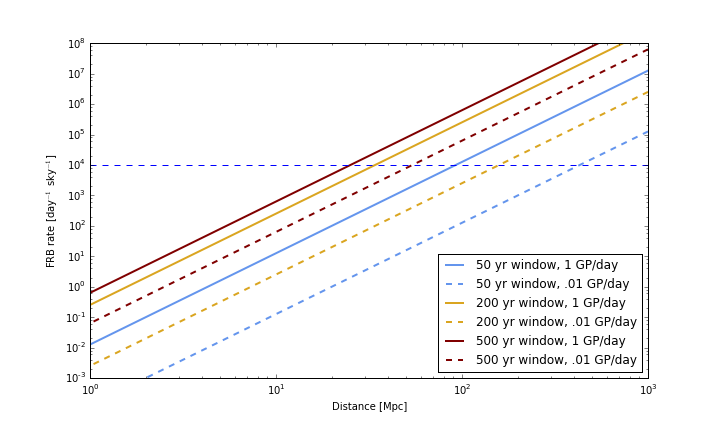
\includegraphics[width=0.5\textwidth]{FRB_SNR_rate.png}
   \caption{Daily FRB rate per sky based on local core-collapse supernova 
   event rate, plotted against distance.
   We assume early in the pulsar's life there is a window, either 
   25, 100, or 500 years when the SNR can provide a large enough electron 
   column density to explain the high DM's of the observed bursts. We also
   include a rate of giant pulses of either one per day or one per hundred
   days. We have assumed 20$\%$ of core-collapse supernovae leave behind
   a visible pulsar.
   The horizontal black lines are the 1$\sigma$ bounds for the FRB rate
   found by \cite{2015arXiv150500834R}.}
   \label{FIG-RATE}
\end{figure}

From this figure we can see even in our most conservative estimate, when
the SNR only has a 25 year window and emits giant pulses once every
100 days, the volume necessary for the highest daily FRB rate is still non-cosmological.
By this we mean the DM contribution from the IGM is less than $\sim 200$ pc/cm$^3$.
If the SNR FRB's are within a hundred h$^{-1}$ Mpc then DM$_{IGM}$ is less than 
$\sim 10 \%$  of the total dispersion of a typical burst.

If FRB's really are giant pulses then they 
should repeat stochastically, and while none of the radio follow-ups for
observed sources has seen an FRB repeat, this could be because they
have not observed for long enough. We discuss this further in section 
\ref{sec-predictions}.

\subsection{Young SNR Pulsars}

About a dozen pulsars in our galaxy are known to emit extremely energetic,
short duration radio pulses which can be many orders of magnitude 
brighter than the pulsar's regular emission. Some of these objects exhibit 
a rare tail of \textit{supergiant} pulses, whose brightness temperatures 
exceed the Planck temperature, $\gtrsim10^{32}$ K. Indeed the largest
observed brightness temperature came from a giant pulse from the Crab
, with T$_b\sim2\times10^{41}$  \citep{2014ApJ...792..135T}.

Given the relatively high frequency of core-collapse supernovae 
in the local universe, the young 
rapidly rotating pulsars such events leave behind could emit giant 
pulses bright enough to be observed at hundreds of megaparsecs. 
These supergiant pulses would require 10^{36 - 37}$ ergs of output,
assuming and observed flux density of 0.3-5 Jy and $\sim500$ 
MHz of bandwidth over 1 ms. Though this is $\sim$ billions of times
brighter than an average pulse, it is negligible compared to a 
pulsar's total rotational energy, E$_{rot} \sim 10^{49-50}$ ergs. We
also point out that given its relative proximity, this model requires
a couple orders of magnitude less energy than cosmological FRB's,
located beyond a Gpc. 

The polarization properties of giant pulses are also consistent with
observed those of FRB's. Giant pulses are known to be highly polarized, 
switching between strong Stokes V and purely linearly polarized states. 
The only published FRB with full-pol information was FRB 140514 was 
found to have $\sim20\%$ circular polarization and no detectable 
linear polarization \citep{2014arXiv1412.0342P}.

\section{Predictions}
\label{sec-predictions}

The young SNR pulsar model makes several predictions that will
be addressed with more data, particularly with full polarization 
observations and large field-of-view surveys. 
The latter will provide a large sample of FRB's whose flux and DM statistics
that can give us information about their location. Since in the SNR FRB picture
most of the DM is intrinsic, the sources do not need to be at cosmological 
distances. This means the flux distribution is given by a Euclidean universe
that is only weakly dependent on DM ($N(S) \propto$ $S^{-5/2}$). Surveys
like CHIME \citep{2014SPIE.9145E..22B}, 
UTMOST\footnote{http://www.caastro.org/news/2014-utmost},
 or HYRAX could observe as many as $\sim10^{3-4}$
per year, which would allow for detailed population statistics.
\\
Since we have proposed that FRB's come from young pulsars 
in supernova remnants, it is possible that the corresponding 
supernova was observed in recent decades in the optical. If the pulsars
were younger than $\sim$60 years old they could be localized with VLBI
measurements and matched against catalogued type II supernovae. 
\\
We also point out that while FRB's seem not to repeat regularly, 
it is not known that they never repeat. Though the statistics 
of giant pulses from local pulsars are mostly Poisson \citep{1999ApJ...517..460S},
it is possible that 
the supergiant pulses we require from very young SNR pulsars are not. If their 
statistics were of a Poisson process then there are already limits on the repeat rate, 
given the $\sim100$ hours of follow up, however if their statistics were more like
earthquakes, the brightest pulses could burst intermittently and turn off
for extended periods. It is possible that FRB's could repeat every 5-500 days. 
If they were to repeat,
it is possible that their DM's, RM's, and scattering properties could 
change noticeably on months/years timescales. Unlike standard pulsars 
whose RM's and DM's are constant to a couple decimal places, young 
SNR pulsars like the Crab and Vela have shown significant - and sometimes
correlated - variation in such properties \citep{1988A&A...202..166R, 2008A&A...483...13K}.
. We also predict that such repeated 
bursts could have vastly different polarization states, similar to the giant 
pulses from pulsars in our own galaxy.
\\
Finally, depending on the relationship between the giant pulse rate and SNR
age and environment, there may exist a short window in the pulsar's life when 
DM's are larger than could be achieved in the IGM. It would be therefore 
possible, albeit rare, that an FRB have a dispersion
 measure of $\sim10^4$ pc/cm$^3$.

%\section{Applications}

\section{Conclusions}
Evidence is piling on suggesting FRB's are not only extraterrestrial
but extragalactic. Though the simplest interpretation of their high DM's 
is a cosmological one, we find this model less compelling in the light of 
scattering and polarization measurements, and in this letter we offer a 
more nearby solution. We have gone through
a model in which fast radio bursts are really supergiant pulses from 
extragalactic supernova remnant pulsars, within a couple hundred megaparsecs. 
The SNR environment is sufficiently
dense and ionized to provide DM's $\gtrsim 300$pc/cm$^3$ as well as 
RM's $\gtrsim 100$ rad/m$^2$, only the first of which could be replicated by the IGM. 

The nebula could also provide $\sim$ms scattering at 1GHz, as has been 
observed in galactic supernova remnant pulsars. 
That makes this picture self-contained in the sense that
the young remnant environment can account for the dispersion 
and scattering measure - and perhaps Faraday rotation - seen in FRB's. 
By extrapolating Crab-like giant pulses back to the pulsar's first century or so,
we have proposed that such objects can emit extremely energetic bursts sporadically. 
If these are similar to giant pulses from galactic pulsars, they could be highly polarized, 
either linearly or circularly, and if they were to repeat their polarization state may 
change drastically. 

(Include quick summary of predictions)

\section{Acknowledgements}

We thank NSERC for support. We also thank Bryan Gaensler, Neils Oppermann, 
Giovanna Zanardo, and Chris Matzner for helpful discussions. 

%\bibliography{frb}
\bibliography{SNRFRB_April30}
\bibliographystyle{emulateapj}


\label{lastpage}

\end{document}


